\documentclass{scrbook}

\usepackage{graphicx} % includegraphics
\usepackage{pgffor} % foreach

\begin{document}

\chapter{Data Import Preparation}
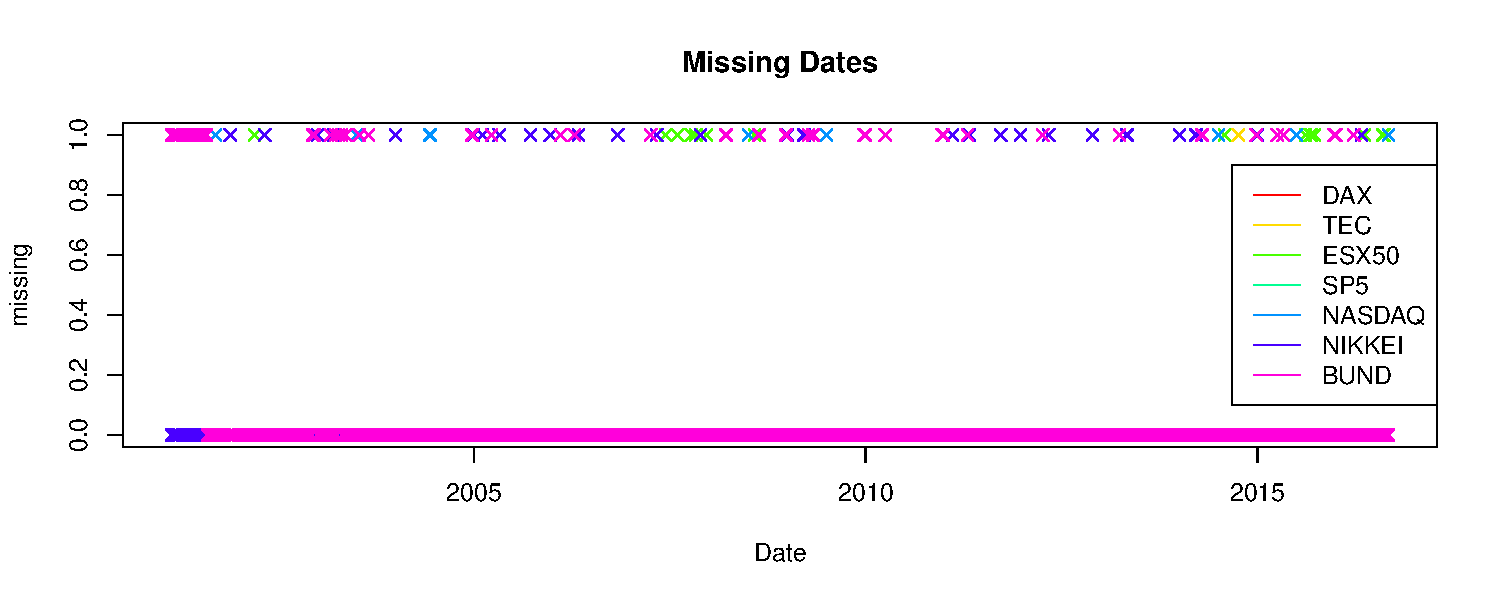
\includegraphics[width=\textwidth]{missingDates.pdf}


\chapter{Data Visualization}
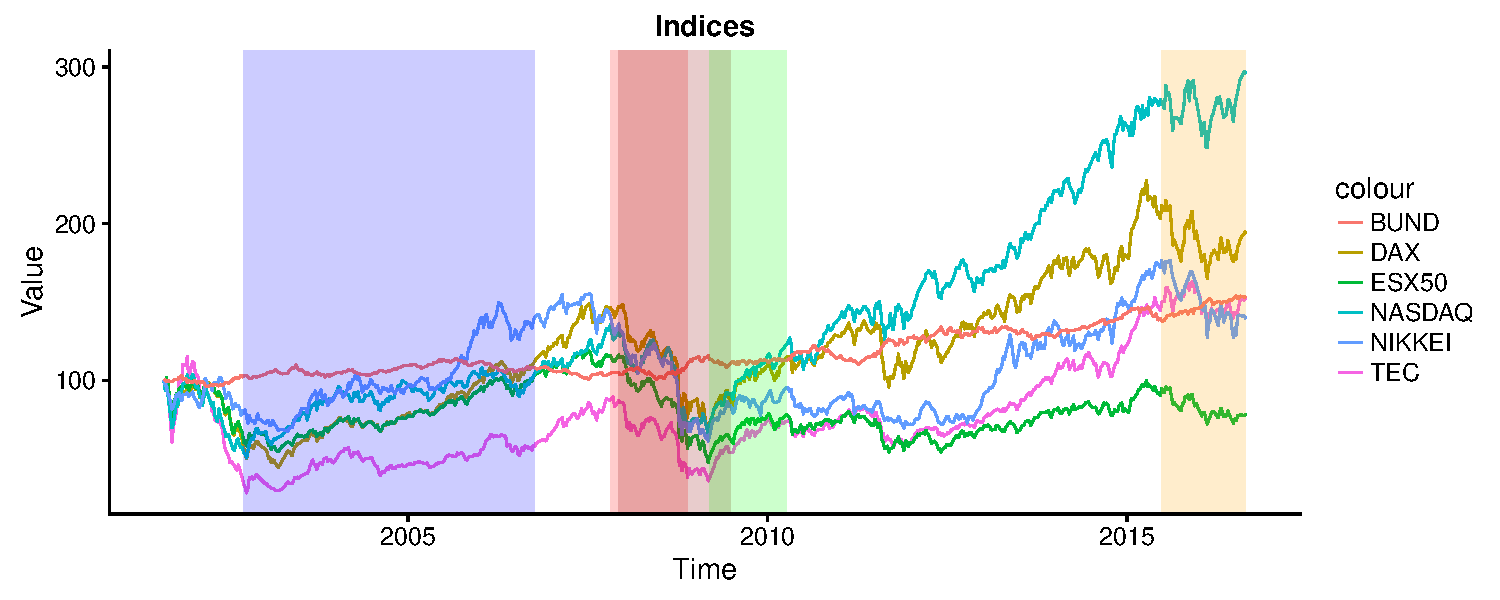
\includegraphics[width=\textwidth]{retPlot.pdf}
\input{0sentixDisp.txt}

\input{0sentixHerf.txt}

\chapter{Results}

\section{Ternary}
\clearpage
\input{0Ternary-Dispersion.txt}

\clearpage
\section{Performance}

\subsection{classic - constant weights}
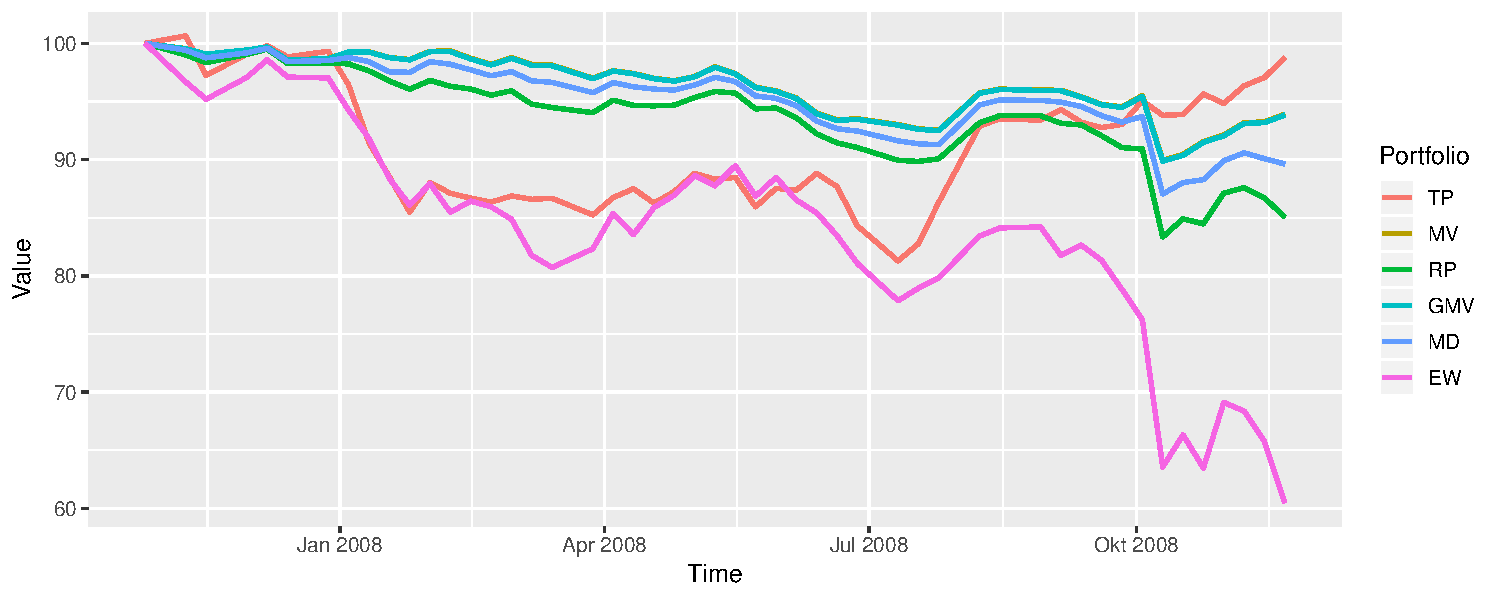
\includegraphics[width=\textwidth]{Performance-Classic-datesEvalBear.pdf}
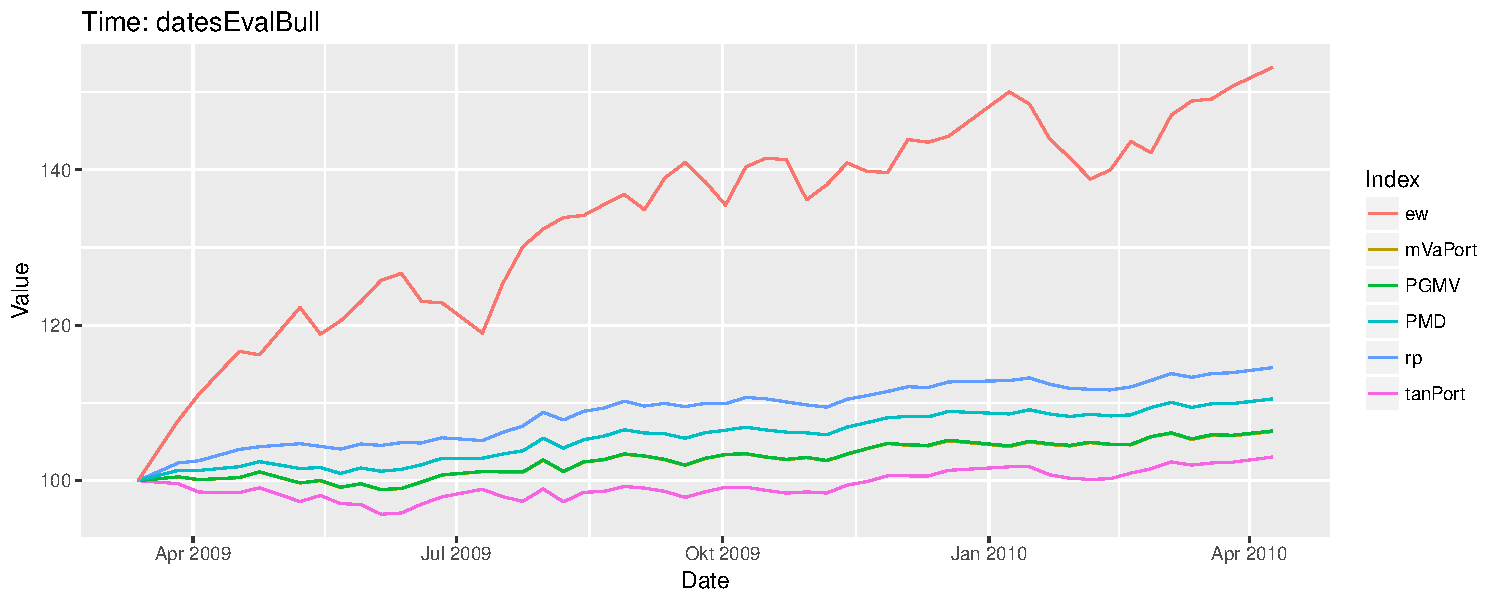
\includegraphics[width=\textwidth]{Performance-Classic-datesEvalBull.pdf}
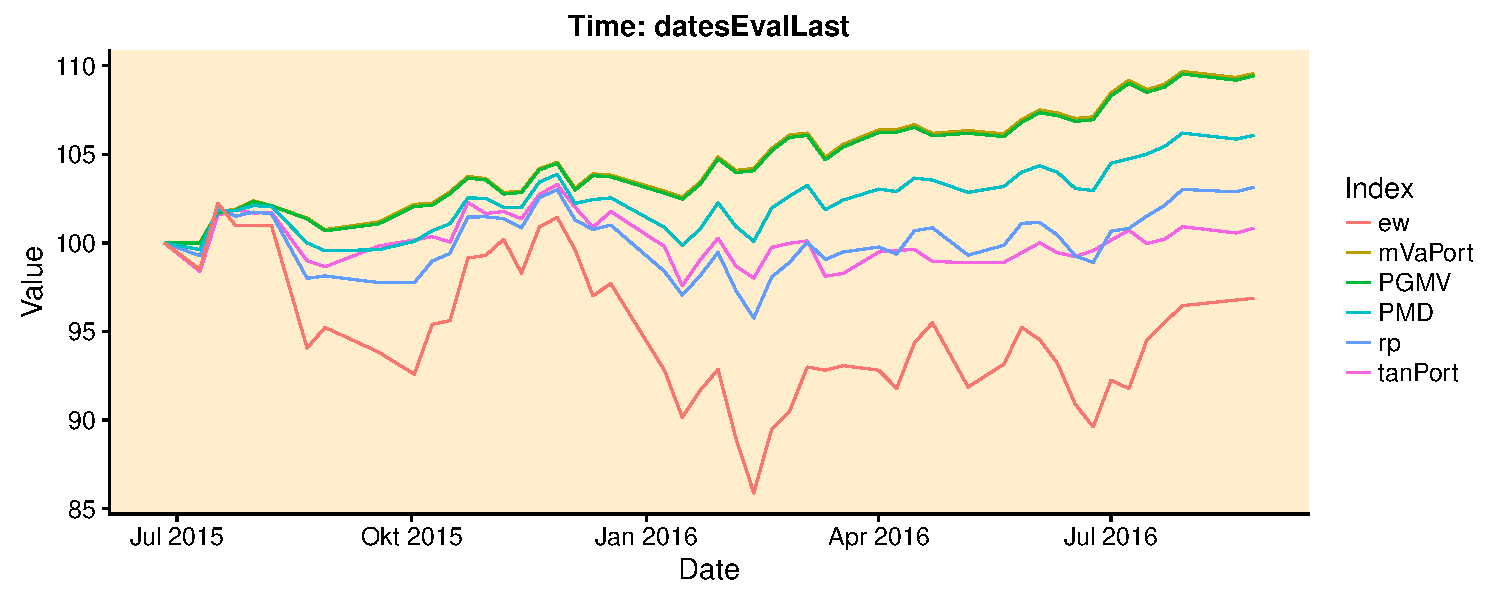
\includegraphics[width=\textwidth]{Performance-Classic-datesEvalLast.pdf}
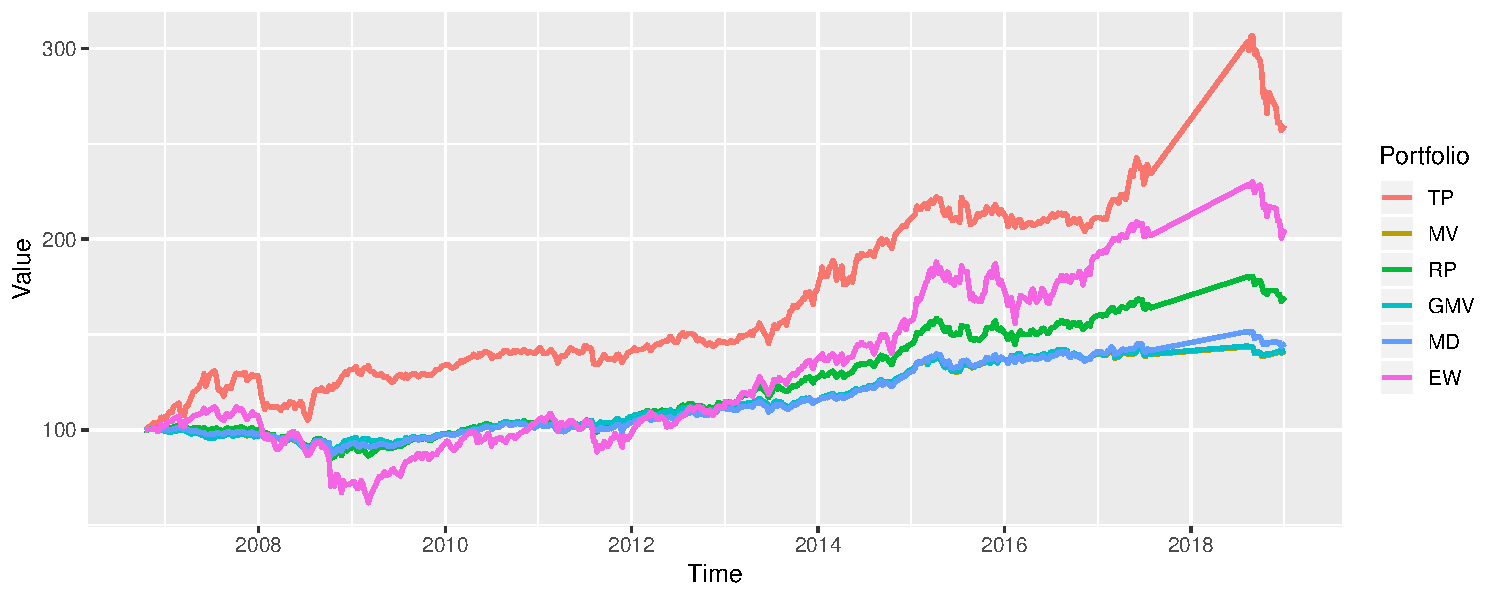
\includegraphics[width=\textwidth]{Performance-Classic-datesEvalAllAfterTest.pdf}

\input{0Performance-Sentix.txt}
\input{0Performance-Classic.txt}
\input{0Performance-Classic-No-Risk-Free.txt}
\input{0Performance-All-classicWithRiskFree.txt}
\input{0Performance-All-classicNoRiskFree.txt}

\clearpage
\section{Analysis}
\input{0Summary-Sentix.txt}
\input{0Summary-Classic.txt}
\input{0Summary-Classic-No-Risk-Free.txt}
\input{0SummaryAll-classicWithRiskFree.txt}
\input{0SummaryAll-classicNoRiskFree.txt}


\clearpage
\section{Weights}
\input{0Weights-Sentix.txt}
\input{0Weights-Classic.txt}
\input{0Weights-Classic-No-Risk-Free.txt}


\end{document}